% Appendix. Figures in figs/supp/ and tables in tabs/supp/ are generated by regenerate_supplementary.py
% from final/results; rerun it after rerunning the experiments. Floats use [H] so that every figure
% and table stays in its subsection.

\begin{center}
  {\LARGE\bfseries Appendix}
\end{center}

All figures and tables of this appendix are produced from the outputs of the experiment scripts. Unless stated otherwise, accuracies are nested-CV means $\pm$ standard deviations over 10 repeats of stratified 5-fold cross-validation, with the LV reconstructed by \emph{fill+hull} for training and evaluated patients.

\startcontents[appendix]
\printcontents[appendix]{}{1}{\setcounter{tocdepth}{2}\section*{Contents}\footnotesize}

\clearpage
% ==========================================================================================
\section{Dataset}
\label{app:data}

\subsection{Patients}
Table~\ref{tab:supp-classes} describes the patients. ARV patients are lighter on average and have more slices, with a smaller slice step; the test set has more slices on average than the training set. All our features are computed in millimeters, so they do not depend on the resolution, but the thickness features are sampled more coarsely along the long axis when the slice step is large.

% Generated by regenerate_supplementary.py from results/dataset/tables/class_stats.csv
\begin{table}[H]
\centering
\small
\setlength{\tabcolsep}{4pt}
\begin{adjustbox}{max width=\linewidth}
\begin{tabular}{lrrrrrr}
\toprule
Group & Patients & Height (cm) & Weight (kg) & Slices & In-plane (mm) & Slice step (mm) \\
\midrule
DCM & 20 & 171.1 & 75.5 & 9.8 & 1.51 & 10.0 \\
HCM & 20 & 169.8 & 80.3 & 9.4 & 1.49 & 9.8 \\
MINF & 20 & 172.2 & 74.2 & 8.7 & 1.49 & 9.8 \\
NOR & 20 & 172.2 & 77.9 & 8.5 & 1.52 & 9.8 \\
ARV & 20 & 168.9 & 66.9 & 11.2 & 1.55 & 7.3 \\
Test (n=50) & 50 & 170.0 & 80.7 & 10.8 & 1.52 & 9.1 \\
\bottomrule
\end{tabular}
\end{adjustbox}
\caption{Patients per class (means). The training set has 20 patients per class; the test set has the same number of patients per class in ACDC, but its labels are not available. Slice counts range from 6 to 21; slice steps take the values 5, 6.5, 7, 10 mm.}
\label{tab:supp-classes}
\end{table}


\clearpage
% ==========================================================================================
\section{Features}
\label{app:features}

\subsection{Definitions and class means}
Table~\ref{tab:supp-features} defines the 32 features and gives their mean per group. Volumes are counted in voxels and multiplied by the voxel volume given in the file header. Wall-thickness samples are read on the Euclidean distance transform of the union of the myocardium and the cavity (filled), at the myocardium pixels that are 4-connected to the cavity, with the in-plane pixel spacing as sampling; slices without myocardium or without cavity are skipped.

% Generated by regenerate_supplementary.py from final/cache/features/train_fill_hull.csv
\begin{table}[H]
\centering
\scriptsize
\setlength{\tabcolsep}{4pt}
\begin{adjustbox}{max width=\linewidth}
\begin{tabular}{lp{0.4\linewidth}crrrrr}
\toprule
Feature & Definition & Set & NOR & MINF & DCM & HCM & ARV \\
\midrule
\texttt{ed\_lv\_vol} & LV volume at ED (mL) & V & 130.1 & 172.2 & 284.6 & 129.3 & 107.1 \\
\texttt{es\_lv\_vol} & LV volume at ES (mL) & V & 51.7 & 119.4 & 233.1 & 42.2 & 49.1 \\
\texttt{lv\_ef} & LV ejection fraction, $100\,(V_{ED}-V_{ES})/V_{ED}$ (\%) & V, C & 60.3 & 31.0 & 18.5 & 67.4 & 54.7 \\
\texttt{ed\_rv\_vol} & RV volume at ED (mL) & V & 153.2 & 119.1 & 178.0 & 118.3 & 196.3 \\
\texttt{es\_rv\_vol} & RV volume at ES (mL) & V & 68.8 & 54.7 & 125.6 & 46.1 & 134.1 \\
\texttt{rv\_ef} & RV ejection fraction (\%) & V, C & 55.1 & 55.5 & 31.8 & 59.8 & 31.4 \\
\texttt{myocardium\_mass} & Myocardial mass, $1.05$ g/mL $\times$ volume, mean of ED and ES (g) & V & 111.0 & 131.5 & 176.9 & 191.3 & 82.7 \\
\texttt{lv\_mass\_index} & Myocardial mass / BSA (g/m$^2$) & V, C & 57.6 & 70.3 & 95.8 & 99.4 & 46.5 \\
\texttt{stroke\_volume} & LV stroke volume, $V_{ED}-V_{ES}$ (mL) & V & 78.4 & 52.8 & 51.5 & 87.1 & 58.0 \\
\texttt{es\_lv\_index} & LV ES volume / BSA & V, C & 26.9 & 64.1 & 125.6 & 22.0 & 27.6 \\
\texttt{ed\_rv\_index} & RV ED volume / BSA & V, C & 79.6 & 63.3 & 94.2 & 60.9 & 111.9 \\
\texttt{ratio\_rv\_lv\_es} & RV / LV volume at ES & V & 1.33 & 0.49 & 0.53 & 1.17 & 3.16 \\
\texttt{ratio\_rv\_lv\_ed} & RV / LV volume at ED & V, C & 1.17 & 0.72 & 0.62 & 0.93 & 2.00 \\
\texttt{weight} & Weight (kg) & V & 77.9 & 74.2 & 75.5 & 80.3 & 66.9 \\
\texttt{height} & Height (cm) & V & 172.2 & 172.2 & 171.1 & 169.8 & 168.9 \\
\texttt{bsa} & Body surface area, Mosteller (m$^2$) & V & 1.92 & 1.88 & 1.88 & 1.94 & 1.76 \\
\texttt{ed\_lv\_index} & LV ED volume / BSA & V, C & 67.8 & 92.4 & 153.4 & 67.3 & 60.2 \\
\texttt{es\_rv\_index} & RV ES volume / BSA & V, C & 35.6 & 29.0 & 66.3 & 24.0 & 76.5 \\
\texttt{myocardium\_to\_lv\_ed} & ED myocardial mass / LV ED volume & V & 0.79 & 0.74 & 0.60 & 1.40 & 0.75 \\
\texttt{mass\_to\_edv\_ratio} & Mean myocardial mass / LV ED volume & V, C & 0.86 & 0.79 & 0.63 & 1.51 & 0.80 \\
\texttt{mass\_ratio\_systole\_diastole} & ES / ED myocardial mass & V & 1.17 & 1.14 & 1.08 & 1.18 & 1.15 \\
\texttt{ed\_thick\_mean} & ED wall thickness, mean over all samples (mm) & T & 7.12 & 7.45 & 7.52 & 10.6 & 6.24 \\
\texttt{ed\_thick\_max} & ED wall thickness, maximum sample (mm) & T & 11.7 & 13.7 & 12.4 & 20.8 & 11.5 \\
\texttt{ed\_thick\_slicemean\_max} & ED wall thickness, largest per-slice mean (mm) & T, C & 8.39 & 9.24 & 8.70 & 13.0 & 7.51 \\
\texttt{ed\_thick\_slicestd\_mean} & ED wall thickness, mean of per-slice std (mm) & T, C & 1.19 & 1.64 & 1.40 & 2.44 & 1.25 \\
\texttt{ed\_thick\_slicemean\_std} & ED wall thickness, std of per-slice means (mm) & T & 1.03 & 1.36 & 0.96 & 2.04 & 0.96 \\
\texttt{es\_thick\_mean} & ES wall thickness, mean over all samples (mm) & T & 11.4 & 9.34 & 8.79 & 17.0 & 9.44 \\
\texttt{es\_thick\_max} & ES wall thickness, maximum sample (mm) & T & 16.9 & 19.0 & 14.7 & 25.7 & 15.3 \\
\texttt{es\_thick\_slicemean\_max} & ES wall thickness, largest per-slice mean (mm) & T & 13.4 & 13.0 & 10.2 & 20.0 & 11.4 \\
\texttt{es\_thick\_slicestd\_mean} & ES wall thickness, mean of per-slice std (mm) & T & 1.70 & 2.57 & 1.69 & 2.64 & 1.68 \\
\texttt{es\_thick\_slicemean\_std} & ES wall thickness, std of per-slice means (mm) & T & 1.63 & 2.54 & 1.03 & 2.64 & 1.60 \\
\texttt{wall\_thickening} & Systolic thickening, ES / ED mean thickness & T, C & 1.60 & 1.26 & 1.17 & 1.60 & 1.52 \\
\bottomrule
\end{tabular}
\end{adjustbox}
\caption{The 32 features and their mean per class (training set, reconstructed LV). \emph{Set}: V = volumetric, T = wall thickness, C = compact set. Volumes in mL, indices per m$^2$ of BSA.}
\label{tab:supp-features}
\end{table}


\subsection{Thickness features per group}
HCM has the thickest walls on every descriptor (Figure~\ref{fig:supp-thick}). MINF has walls of normal mean thickness at ED but, with HCM, the most uneven walls at ES, and its systolic thickening is low, as is that of DCM: both groups have a poorly contracting LV, but only MINF has a wall that is uneven along its circumference.

\begin{figure}[H]
  \centering
  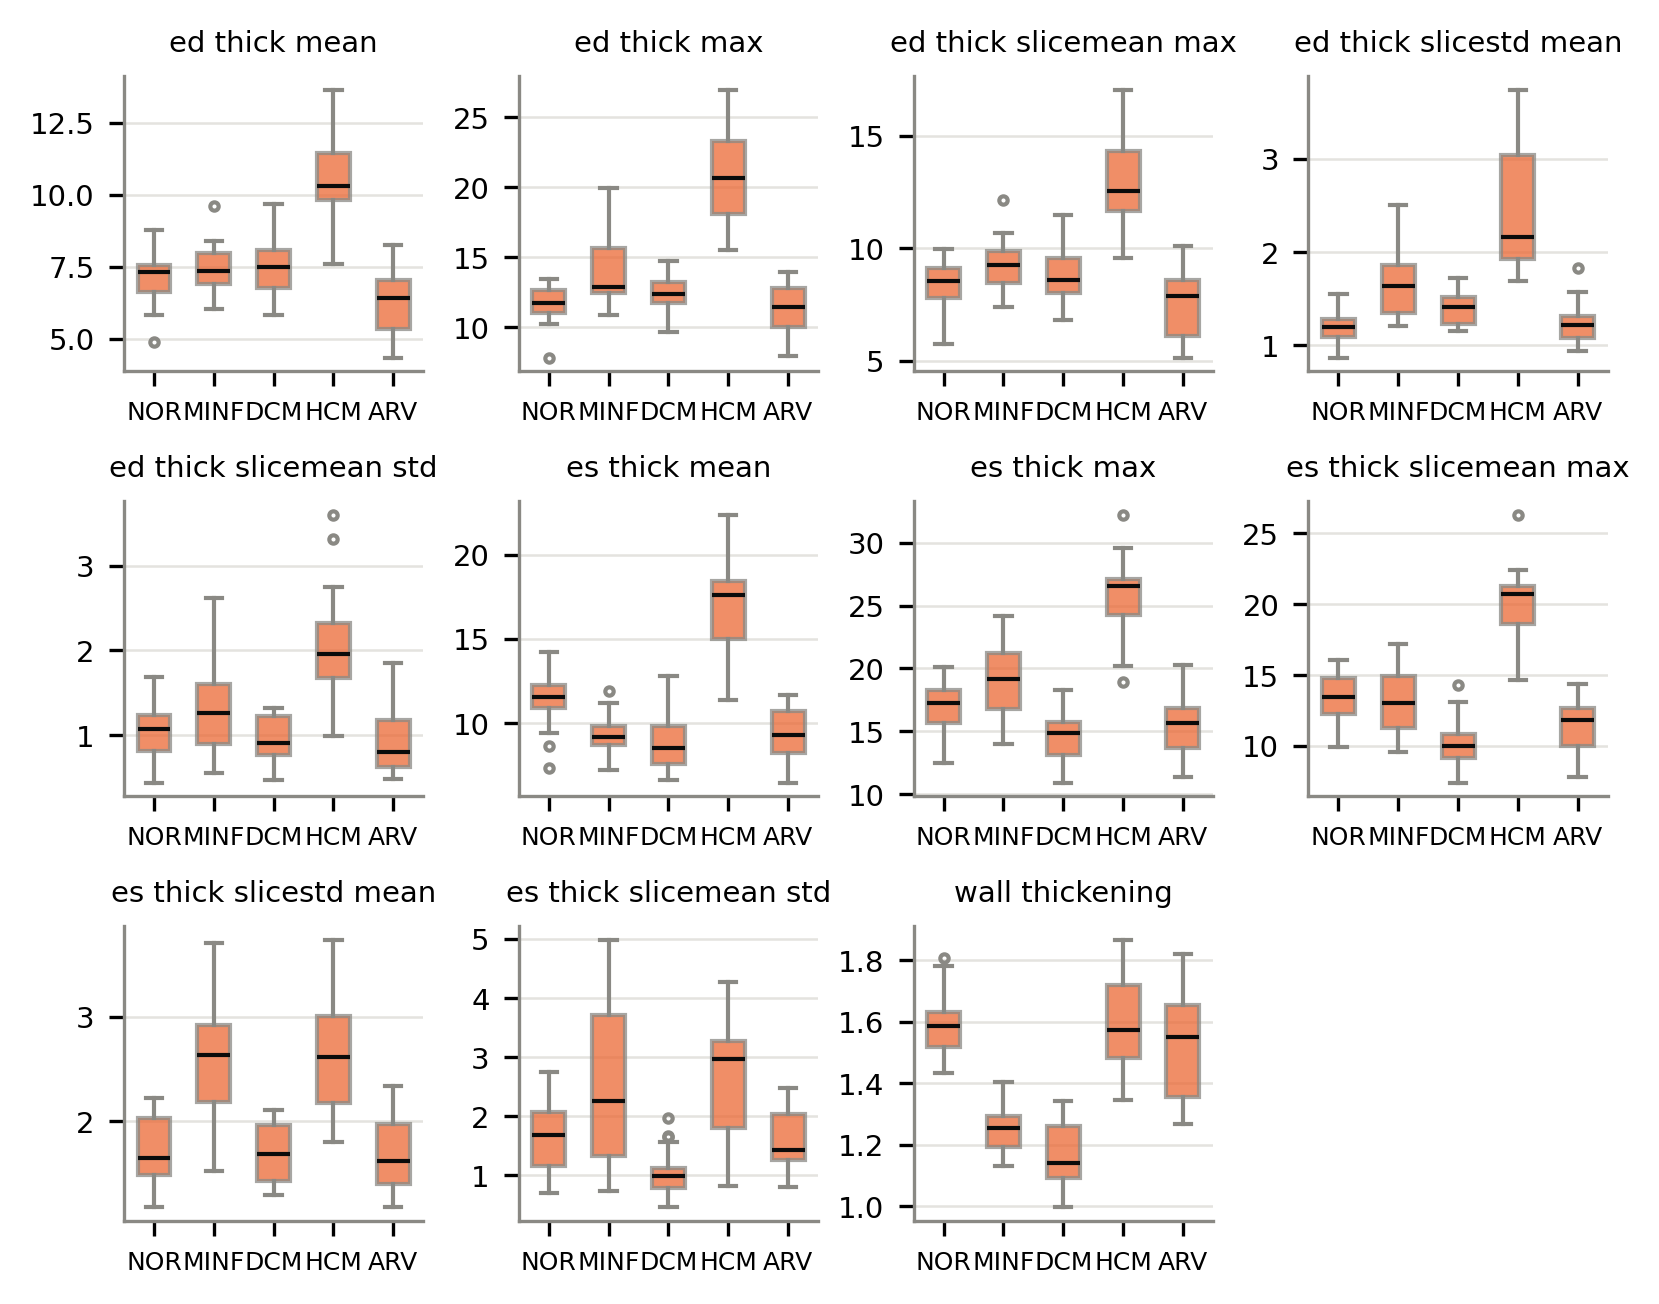
\includegraphics[width=\linewidth]{figs/supp/thickness_by_class.png}
  \caption{Distribution of the 11 thickness features per group (training set, reconstructed LV).}
  \label{fig:supp-thick}
\end{figure}

\clearpage
% ==========================================================================================
\section{Reconstruction of the LV cavity}
\label{app:lv}

\subsection{Volumes not reconstructed exactly}
Table~\ref{tab:supp-lv} lists the 7 training volumes that the filling does not reconstruct exactly. With the convex-hull fallback, the remaining errors are a few boundary voxels of the basal slice (at most 3.1 mL). The filling alone misestimates the ejection fraction of patient 011 by 12 points and of patient 069 by 13 points.

% Generated by regenerate_supplementary.py from results/lv_reconstruction/tables/per_volume.csv
\begin{table}[H]
\centering
\scriptsize
\setlength{\tabcolsep}{4pt}
\begin{adjustbox}{max width=\linewidth}
\begin{tabular}{lllrrrrrrr}
\toprule
Patient & Phase & Class & True LV (mL) & \multicolumn{2}{c}{Filling: $\Delta V$, Dice} & \multicolumn{2}{c}{+ convex hull: $\Delta V$, Dice} & \multicolumn{2}{c}{$\Delta$EF (points)} \\
\midrule
011 & ED & DCM & 237.0 & $-$28.7 & 0.935 & 1.2 & 0.998 & $-$12.1 & 0.4 \\
045 & ES & MINF & 158.6 & $-$25.7 & 0.912 & 1.2 & 0.996 & 11.4 & $-$0.5 \\
029 & ED & HCM & 157.1 & $-$10.8 & 0.965 & 3.1 & 0.990 & $-$1.3 & 0.4 \\
069 & ES & NOR & 33.3 & $-$9.6 & 0.832 & 0.6 & 0.991 & 12.8 & $-$0.8 \\
068 & ES & NOR & 49.3 & $-$9.5 & 0.893 & 0.8 & 0.992 & 7.7 & $-$0.6 \\
096 & ES & ARV & 74.9 & $-$7.3 & 0.949 & 0.4 & 0.998 & 4.8 & $-$0.2 \\
084 & ES & ARV & 22.1 & $-$4.0 & 0.901 & 0.1 & 0.997 & 7.0 & $-$0.2 \\
\bottomrule
\end{tabular}
\end{adjustbox}
\caption{The training volumes that the filling does not reconstruct exactly. Each one misses its most basal slice (slice 0, or 1 for patient 096), where the myocardium does not close around the cavity. The two $\Delta$EF columns are for the filling and for the filling with the convex-hull fallback.}
\label{tab:supp-lv}
\end{table}


\subsection{Effect on the features}
Table~\ref{tab:supp-shift} gives the largest change of each feature when the training LV is reconstructed instead of taken from the ground truth. With the fallback, the volumes and ejection fractions are almost unchanged; the thickness descriptors of the basal slice still change for a few patients, because the reconstructed cavity of that slice is not exactly the true one.

% Generated by regenerate_supplementary.py from results/features/tables/lv_source_shift.csv
\begin{table}[H]
\centering
\small
\setlength{\tabcolsep}{4pt}
\begin{adjustbox}{max width=\linewidth}
\begin{tabular}{lrr}
\toprule
Feature & Filling & + convex hull \\
\midrule
\texttt{stroke\_volume} & 98.5 & 4.0 \\
\texttt{lv\_ef} & 98.3 & 3.5 \\
\texttt{ratio\_rv\_lv\_es} & 40.4 & 1.8 \\
\texttt{es\_lv\_index} & 28.8 & 1.8 \\
\texttt{es\_lv\_vol} & 28.8 & 1.8 \\
\texttt{es\_thick\_slicestd\_mean} & 16.5 & 7.2 \\
\texttt{es\_thick\_slicemean\_std} & 14.5 & 37.5 \\
\texttt{mass\_to\_edv\_ratio} & 13.8 & 1.9 \\
\texttt{ratio\_rv\_lv\_ed} & 13.8 & 1.9 \\
\texttt{myocardium\_to\_lv\_ed} & 13.8 & 1.9 \\
\bottomrule
\end{tabular}
\end{adjustbox}
\caption{Largest relative change (\%, over the 100 training patients) of a feature when the LV is reconstructed instead of taken from the ground truth. Only 7 patients change at all; the ejection fraction of one of them changes by 98\% with the filling.}
\label{tab:supp-shift}
\end{table}


\clearpage
% ==========================================================================================
\section{Protocol study}
\label{app:protocol}

\subsection{Scores of the grids on a single split}
On a single split, most grid configurations obtain the same accuracy, or differ by one patient (Figure~\ref{fig:supp-grid}). The best configuration is therefore determined by one or two patients of one split.

\begin{figure}[H]
  \centering
  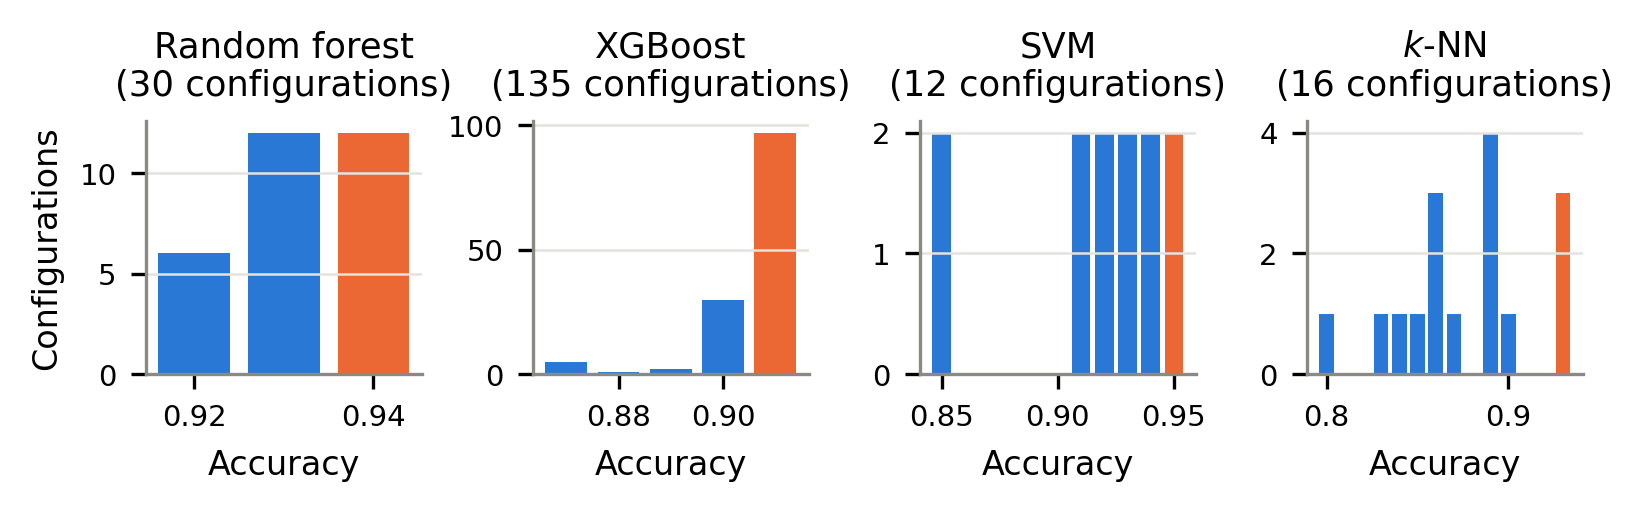
\includegraphics[width=\linewidth]{figs/supp/grid_scores.png}
  \caption{Number of configurations of each grid per accuracy on a single 5-fold split (21 volumetric features, scaler fitted on all patients). Orange: best accuracy, the one a single-split protocol reports.}
  \label{fig:supp-grid}
\end{figure}

\subsection{MLPs scored on their training patients}
Scored on the patients they were trained on, MLP ensembles reach 100\% whatever the number of epochs, so this score cannot select hyper-parameters (Table~\ref{tab:supp-mlp}).

% Generated by regenerate_supplementary.py from results/protocol_study/tables/mlp_training_vs_cv.csv
\begin{table}[H]
\centering
\small
\setlength{\tabcolsep}{4pt}
\begin{adjustbox}{max width=\linewidth}
\begin{tabular}{rrr}
\toprule
Epochs & Accuracy on its training patients & 5-fold CV accuracy \\
\midrule
100 & 1.00 & 0.93 \\
200 & 1.00 & 0.92 \\
500 & 1.00 & 0.93 \\
\bottomrule
\end{tabular}
\end{adjustbox}
\caption{Ensemble of 10 MLPs (same architecture as the final ensemble, learning rate $10^{-3}$, batch 30, 75\% of the patients per MLP), scored on the patients it was trained on and by cross-validation.}
\label{tab:supp-mlp}
\end{table}


\subsection{Feature selection before the cross-validation}
% Generated by regenerate_supplementary.py from results/protocol_study/tables/feature_selection_leak.csv
\begin{table}[H]
\centering
\small
\setlength{\tabcolsep}{4pt}
\begin{adjustbox}{max width=\linewidth}
\begin{tabular}{lr}
\toprule
Random forest (200 trees) & Accuracy \\
\midrule
All 21 features & 0.925 $\pm$ 0.010 \\
Top 16, selected on all patients & 0.924 $\pm$ 0.012 \\
Top 16, selected inside each training fold & 0.923 $\pm$ 0.013 \\
\bottomrule
\end{tabular}
\end{adjustbox}
\caption{Feature selection by random-forest importance, 10 random 5-fold splits (mean $\pm$ std). Selecting on all patients leaks the evaluation folds, but the effect is negligible here.}
\label{tab:supp-selection}
\end{table}


\clearpage
% ==========================================================================================
\section{Benchmark: full results}
\label{app:bench}

\subsection{All configurations}
Table~\ref{tab:supp-benchmark} gives the accuracy, the macro-F1, the recall of each group and the paired difference with the best configuration. NOR is the easiest group (recall 0.95 to 1.00 for almost every model); MINF and DCM are the hardest. The compact set favors HCM and penalizes MINF.

% Generated by regenerate_supplementary.py from results/benchmark/tables/summary_mean.csv
\begin{table}[H]
\centering
\scriptsize
\setlength{\tabcolsep}{4pt}
\begin{adjustbox}{max width=\linewidth}
\begin{tabular}{llrrrrrrrr}
\toprule
Features & Model & Accuracy & Macro-F1 & \multicolumn{5}{c}{Recall: NOR, MINF, DCM, HCM, ARV} & $\Delta$ vs best \\
\midrule
Volumetric & Logistic regression & 0.896 $\pm$ 0.016 & 0.897 & 0.92 & 0.91 & 0.86 & 0.89 & 0.90 & $-$0.070 $\pm$ 0.017 \\
 & Linear SVM & 0.925 $\pm$ 0.016 & 0.925 & 1.00 & 0.94 & 0.86 & 0.87 & 0.94 & $-$0.041 $\pm$ 0.019 \\
 & RBF SVM & 0.923 $\pm$ 0.022 & 0.923 & 0.94 & 0.94 & 0.91 & 0.91 & 0.92 & $-$0.043 $\pm$ 0.025 \\
 & $k$-NN & 0.895 $\pm$ 0.010 & 0.897 & 1.00 & 0.92 & 0.89 & 0.87 & 0.80 & $-$0.071 $\pm$ 0.014 \\
 & Random forest & 0.923 $\pm$ 0.016 & 0.923 & 0.97 & 0.88 & 0.89 & 0.94 & 0.94 & $-$0.043 $\pm$ 0.018 \\
 & Extra trees & 0.931 $\pm$ 0.010 & 0.931 & 0.99 & 0.92 & 0.91 & 0.93 & 0.91 & $-$0.035 $\pm$ 0.012 \\
 & XGBoost & 0.920 $\pm$ 0.013 & 0.920 & 0.96 & 0.88 & 0.91 & 0.94 & 0.91 & $-$0.046 $\pm$ 0.014 \\
 & MLP ensemble & 0.920 $\pm$ 0.012 & 0.921 & 0.97 & 0.94 & 0.89 & 0.89 & 0.91 & $-$0.046 $\pm$ 0.014 \\
 & MLP + RF & 0.925 $\pm$ 0.012 & 0.926 & 1.00 & 0.93 & 0.88 & 0.91 & 0.92 & $-$0.041 $\pm$ 0.014 \\
 & MLP + linear SVM & 0.927 $\pm$ 0.012 & 0.928 & 0.99 & 0.94 & 0.88 & 0.91 & 0.91 & $-$0.039 $\pm$ 0.014 \\
\midrule
Volumetric + thickness & Logistic regression & 0.953 $\pm$ 0.014 & 0.953 & 0.99 & 0.95 & 0.95 & 0.94 & 0.93 & $-$0.013 $\pm$ 0.015 \\
 & Linear SVM & 0.956 $\pm$ 0.014 & 0.956 & 0.97 & 0.95 & 0.93 & 0.97 & 0.94 & $-$0.010 $\pm$ 0.009 \\
 & RBF SVM & 0.945 $\pm$ 0.012 & 0.945 & 0.95 & 0.94 & 0.93 & 0.97 & 0.94 & $-$0.021 $\pm$ 0.013 \\
 & $k$-NN & 0.902 $\pm$ 0.023 & 0.903 & 0.98 & 0.91 & 0.90 & 0.92 & 0.80 & $-$0.064 $\pm$ 0.029 \\
 & Random forest & 0.938 $\pm$ 0.015 & 0.938 & 1.00 & 0.90 & 0.91 & 0.95 & 0.93 & $-$0.028 $\pm$ 0.017 \\
 & Extra trees & 0.937 $\pm$ 0.012 & 0.937 & 0.99 & 0.91 & 0.94 & 0.95 & 0.90 & $-$0.029 $\pm$ 0.015 \\
 & XGBoost & 0.916 $\pm$ 0.021 & 0.916 & 0.99 & 0.86 & 0.91 & 0.94 & 0.89 & $-$0.050 $\pm$ 0.022 \\
 & MLP ensemble & 0.957 $\pm$ 0.008 & 0.957 & 0.99 & 0.95 & 0.93 & 0.95 & 0.95 & $-$0.009 $\pm$ 0.008 \\
 & MLP + RF & 0.954 $\pm$ 0.010 & 0.954 & 1.00 & 0.95 & 0.93 & 0.95 & 0.94 & $-$0.012 $\pm$ 0.012 \\
 & MLP + linear SVM & 0.966 $\pm$ 0.011 & 0.966 & 0.98 & 0.95 & 0.94 & 0.97 & 0.97 & 0.000 $\pm$ 0.000 \\
\midrule
Compact & Logistic regression & 0.942 $\pm$ 0.015 & 0.942 & 0.99 & 0.89 & 0.89 & 1.00 & 0.94 & $-$0.024 $\pm$ 0.015 \\
 & Linear SVM & 0.927 $\pm$ 0.009 & 0.927 & 1.00 & 0.91 & 0.85 & 0.95 & 0.93 & $-$0.039 $\pm$ 0.009 \\
 & RBF SVM & 0.944 $\pm$ 0.019 & 0.944 & 0.99 & 0.89 & 0.91 & 1.00 & 0.93 & $-$0.022 $\pm$ 0.021 \\
 & $k$-NN & 0.932 $\pm$ 0.012 & 0.932 & 0.99 & 0.90 & 0.97 & 0.96 & 0.83 & $-$0.034 $\pm$ 0.015 \\
 & Random forest & 0.925 $\pm$ 0.019 & 0.925 & 1.00 & 0.88 & 0.88 & 0.98 & 0.89 & $-$0.041 $\pm$ 0.022 \\
 & Extra trees & 0.940 $\pm$ 0.009 & 0.940 & 0.99 & 0.91 & 0.94 & 0.99 & 0.86 & $-$0.026 $\pm$ 0.014 \\
 & XGBoost & 0.915 $\pm$ 0.022 & 0.915 & 0.98 & 0.88 & 0.88 & 0.98 & 0.85 & $-$0.051 $\pm$ 0.023 \\
 & MLP ensemble & 0.953 $\pm$ 0.014 & 0.953 & 1.00 & 0.90 & 0.93 & 0.99 & 0.94 & $-$0.013 $\pm$ 0.018 \\
 & MLP + RF & 0.952 $\pm$ 0.019 & 0.952 & 1.00 & 0.90 & 0.93 & 0.98 & 0.94 & $-$0.014 $\pm$ 0.023 \\
 & MLP + linear SVM & 0.955 $\pm$ 0.008 & 0.955 & 1.00 & 0.91 & 0.92 & 0.98 & 0.97 & $-$0.011 $\pm$ 0.014 \\
\bottomrule
\end{tabular}
\end{adjustbox}
\caption{All configurations of the benchmark (nested CV, 10 repeats, reconstructed LV). $\Delta$ vs best: per-repeat difference with the best configuration (MLP + linear SVM, volumetric + thickness), mean $\pm$ std; since all configurations share the same splits, this paired difference is less noisy than the accuracies themselves.}
\label{tab:supp-benchmark}
\end{table}


\subsection{Recall per group}
\begin{figure}[H]
  \centering
  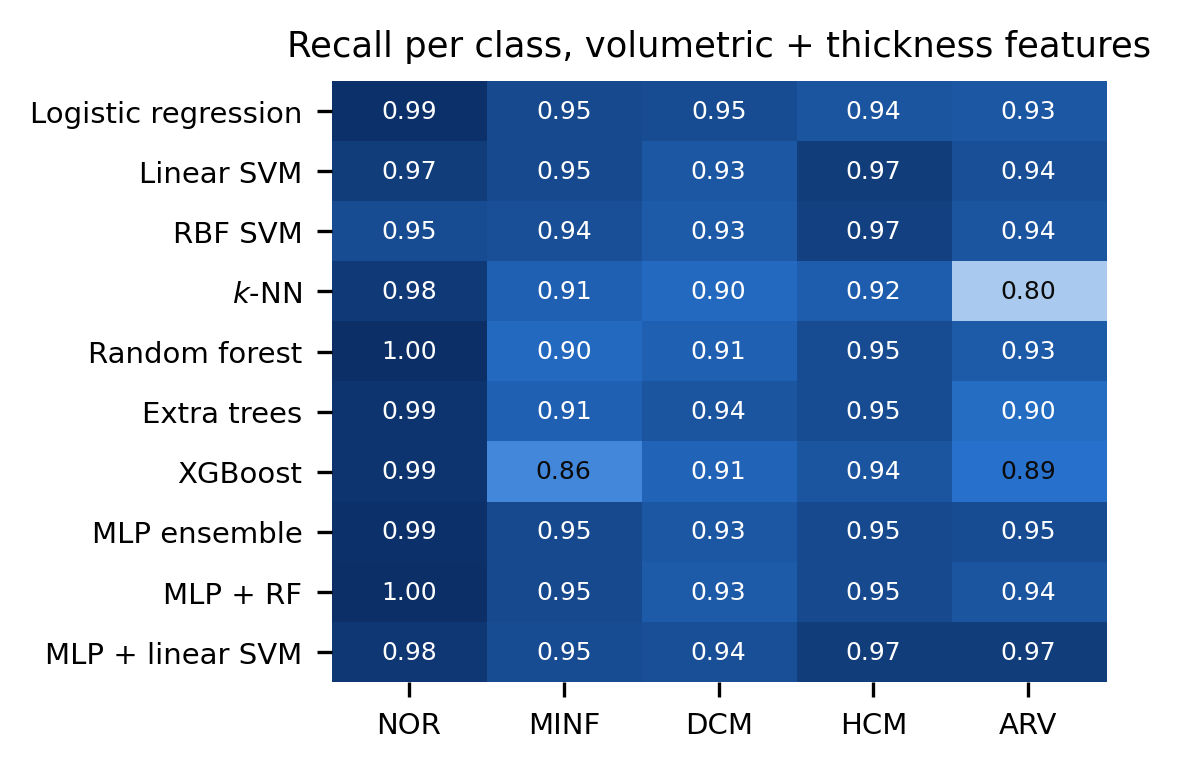
\includegraphics[width=0.62\linewidth]{figs/supp/recall_heatmap.png}
  \caption{Recall of each group for the 10 classifiers on the 32 features (volumetric + thickness).}
  \label{fig:supp-recall}
\end{figure}

\subsection{Hyper-parameters}
The inner cross-validation chooses stable values for the forests (fully grown trees, $\sqrt{d}$ features per split) and XGBoost (shallow trees, column subsampling), and less stable ones for the regularization of the linear models, whose accuracy is flat over a wide range of $C$ (Table~\ref{tab:supp-hyper}). For the soft votes, $\alpha=0.5$ is the most frequent choice, but in less than half of the folds for 5 of the 6 ensembles: this suggests that the inner cross-validation often finds several values of $\alpha$ tied, the tie-breaking rule then picking 0.5.

% Generated by regenerate_supplementary.py from results/benchmark/tables/summary.csv
\begin{table}[H]
\centering
\scriptsize
\setlength{\tabcolsep}{4pt}
\begin{adjustbox}{max width=\linewidth}
\begin{tabular}{llp{0.58\linewidth}}
\toprule
Features & Model & Most frequent choice of the inner CV (count over the 50 outer folds) \\
\midrule
Volumetric & Logistic regression & C=0.01 (14/50) \\
Volumetric & Linear SVM & C=0.1 (33/50) \\
Volumetric & RBF SVM & C=10 (27/50), gamma=scale (25/50) \\
Volumetric & $k$-NN & metric=manhattan (47/50), n\_neighbors=3 (26/50), weights=distance (31/50) \\
Volumetric & Random forest & max\_depth=None (48/50), max\_features=sqrt (43/50) \\
Volumetric & Extra trees & max\_depth=None (37/50), max\_features=sqrt (33/50) \\
Volumetric & XGBoost & colsample\_bytree=0.6 (47/50), learning\_rate=0.05 (44/50), max\_depth=2 (30/50), n\_estimators=100 (35/50) \\
Volumetric & MLP + RF & alpha=0.5 (19/50) \\
Volumetric & MLP + linear SVM & alpha=0.5 (24/50) \\
Volumetric + thickness & Logistic regression & C=10.0 (16/50) \\
Volumetric + thickness & Linear SVM & C=0.1 (32/50) \\
Volumetric + thickness & RBF SVM & C=10 (27/50), gamma=scale (30/50) \\
Volumetric + thickness & $k$-NN & metric=manhattan (29/50), n\_neighbors=5 (15/50), weights=distance (30/50) \\
Volumetric + thickness & Random forest & max\_depth=None (44/50), max\_features=sqrt (44/50) \\
Volumetric + thickness & Extra trees & max\_depth=None (29/50), max\_features=sqrt (38/50) \\
Volumetric + thickness & XGBoost & colsample\_bytree=0.6 (46/50), learning\_rate=0.05 (36/50), max\_depth=2 (35/50), n\_estimators=100 (25/50) \\
Volumetric + thickness & MLP + RF & alpha=0.5 (21/50) \\
Volumetric + thickness & MLP + linear SVM & alpha=0.5 (33/50) \\
Compact & Logistic regression & C=0.1 (15/50) \\
Compact & Linear SVM & C=1.0 (19/50) \\
Compact & RBF SVM & C=1 (24/50), gamma=scale (36/50) \\
Compact & $k$-NN & metric=euclidean (43/50), n\_neighbors=3 (39/50), weights=distance (30/50) \\
Compact & Random forest & max\_depth=None (45/50), max\_features=sqrt (45/50) \\
Compact & Extra trees & max\_depth=None (32/50), max\_features=sqrt (41/50) \\
Compact & XGBoost & colsample\_bytree=0.6 (47/50), learning\_rate=0.05 (42/50), max\_depth=3 (25/50), n\_estimators=100 (27/50) \\
Compact & MLP + RF & alpha=0.5 (18/50) \\
Compact & MLP + linear SVM & alpha=0.5 (21/50) \\
\bottomrule
\end{tabular}
\end{adjustbox}
\caption{Hyper-parameters selected by the inner cross-validation. Grids: $C\in\{0.01,0.1,1,10,100\}$ for logistic regression and the linear SVM; $C\in\{0.1,1,10,100\}$, $\gamma\in\{$scale$, 0.01, 0.1\}$ for the RBF SVM; $k\in\{3,5,7,9\}$, uniform or distance weights, Euclidean or Manhattan for $k$-NN; depth $\in\{$none$, 5\}$, features per split $\in\{\sqrt{d}, d/2\}$ for the forests (300 trees); 100 or 300 trees, depth 2 or 3, learning rate 0.05 or 0.1, column subsampling 0.6 or 1 for XGBoost; $\alpha\in\{0,0.1,\dots,1\}$ for the soft votes. A frequent \texttt{None} depth means fully grown trees.}
\label{tab:supp-hyper}
\end{table}


\clearpage
% ==========================================================================================
\section{Final model}
\label{app:final}

\subsection{Repeats and errors}
% Generated by regenerate_supplementary.py from results/final_model/tables/nested_per_repeat.csv
\begin{table}[H]
\centering
\small
\setlength{\tabcolsep}{4pt}
\begin{adjustbox}{max width=\linewidth}
\begin{tabular}{rrrrrrr}
\toprule
Repeat & Accuracy & NOR & MINF & DCM & HCM & ARV \\
\midrule
0 & 0.98 & 1.00 & 0.95 & 0.95 & 1.00 & 1.00 \\
1 & 0.96 & 0.95 & 0.95 & 0.95 & 0.95 & 1.00 \\
2 & 0.97 & 1.00 & 0.95 & 0.95 & 0.95 & 1.00 \\
3 & 0.97 & 1.00 & 0.95 & 0.95 & 1.00 & 0.95 \\
4 & 0.97 & 0.95 & 0.95 & 0.95 & 1.00 & 1.00 \\
5 & 0.96 & 1.00 & 0.95 & 1.00 & 0.95 & 0.90 \\
6 & 0.97 & 1.00 & 0.95 & 0.95 & 0.95 & 1.00 \\
7 & 0.94 & 0.95 & 0.95 & 0.90 & 0.95 & 0.95 \\
8 & 0.97 & 1.00 & 0.95 & 0.90 & 1.00 & 1.00 \\
9 & 0.97 & 1.00 & 0.95 & 0.95 & 1.00 & 0.95 \\
\midrule
Mean & 0.966 $\pm$ 0.011 & 0.985 & 0.950 & 0.945 & 0.975 & 0.975 \\
\bottomrule
\end{tabular}
\end{adjustbox}
\caption{Final model, nested CV: accuracy and recall per class for each of the 10 repeats (100 patients each).}
\label{tab:supp-repeats}
\end{table}

% Generated by regenerate_supplementary.py from results/final_model/tables/misclassified_patients.csv
\begin{table}[H]
\centering
\small
\setlength{\tabcolsep}{4pt}
\begin{adjustbox}{max width=\linewidth}
\begin{tabular}{lllrrrrr}
\toprule
Patient & True & Most predicted & Error rate & LV EF & LV EDV / BSA & ES thick.\ std & RV EF \\
\midrule
050 & MINF & DCM & 1.0 & 16.4 & 162.5 & 2.18 & 72.5 \\
002 & DCM & MINF & 0.9 & 29.1 & 150.7 & 2.06 & 69.5 \\
022 & HCM & HCM & 0.5 & 64.9 & 51.7 & 1.89 & 44.2 \\
015 & DCM & DCM & 0.2 & 25.7 & 123.2 & 1.34 & 46.8 \\
067 & NOR & NOR & 0.2 & 59.7 & 83.6 & 1.50 & 49.3 \\
088 & ARV & ARV & 0.2 & 48.4 & 78.7 & 2.33 & 44.6 \\
089 & ARV & ARV & 0.2 & 62.8 & 34.9 & 1.60 & 10.1 \\
065 & NOR & NOR & 0.1 & 66.0 & 67.9 & 2.07 & 60.7 \\
082 & ARV & ARV & 0.1 & 55.0 & 70.6 & 2.12 & 45.0 \\
\bottomrule
\end{tabular}
\end{adjustbox}
\caption{Patients misclassified in at least one of the 10 repeats of the final model, with four of their features (class means in Table~\ref{tab:supp-features}).}
\label{tab:supp-errors}
\end{table}


\subsection{Permutation importance}
% Generated by regenerate_supplementary.py from results/final_model/tables/permutation_importance.csv
\begin{table}[H]
\centering
\scriptsize
\setlength{\tabcolsep}{4pt}
\begin{adjustbox}{max width=\linewidth}
\begin{tabular}{lrlr}
\toprule
Feature & Accuracy drop & Feature & Accuracy drop \\
\midrule
\texttt{es\_thick\_slicestd\_mean} & 0.050 $\pm$ 0.033 & \texttt{ed\_rv\_vol} & 0.007 $\pm$ 0.015 \\
\texttt{lv\_ef} & 0.025 $\pm$ 0.016 & \texttt{ed\_lv\_index} & 0.006 $\pm$ 0.015 \\
\texttt{rv\_ef} & 0.024 $\pm$ 0.033 & \texttt{es\_thick\_mean} & 0.005 $\pm$ 0.017 \\
\texttt{stroke\_volume} & 0.024 $\pm$ 0.029 & \texttt{es\_thick\_slicemean\_max} & 0.005 $\pm$ 0.020 \\
\texttt{es\_rv\_vol} & 0.019 $\pm$ 0.023 & \texttt{ed\_rv\_index} & 0.005 $\pm$ 0.016 \\
\texttt{ratio\_rv\_lv\_es} & 0.019 $\pm$ 0.023 & \texttt{es\_lv\_index} & 0.005 $\pm$ 0.011 \\
\texttt{myocardium\_mass} & 0.018 $\pm$ 0.024 & \texttt{ed\_thick\_slicemean\_std} & 0.005 $\pm$ 0.015 \\
\texttt{height} & 0.017 $\pm$ 0.018 & \texttt{mass\_to\_edv\_ratio} & 0.004 $\pm$ 0.015 \\
\texttt{lv\_mass\_index} & 0.016 $\pm$ 0.017 & \texttt{es\_thick\_max} & 0.003 $\pm$ 0.024 \\
\texttt{ratio\_rv\_lv\_ed} & 0.015 $\pm$ 0.018 & \texttt{es\_lv\_vol} & 0.003 $\pm$ 0.007 \\
\texttt{es\_rv\_index} & 0.014 $\pm$ 0.026 & \texttt{myocardium\_to\_lv\_ed} & 0.002 $\pm$ 0.016 \\
\texttt{ed\_thick\_max} & 0.013 $\pm$ 0.025 & \texttt{ed\_thick\_mean} & 0.001 $\pm$ 0.021 \\
\texttt{es\_thick\_slicemean\_std} & 0.012 $\pm$ 0.020 & \texttt{ed\_thick\_slicemean\_max} & $-$0.001 $\pm$ 0.011 \\
\texttt{ed\_lv\_vol} & 0.011 $\pm$ 0.021 & \texttt{bsa} & $-$0.001 $\pm$ 0.018 \\
\texttt{wall\_thickening} & 0.011 $\pm$ 0.015 & \texttt{weight} & $-$0.003 $\pm$ 0.012 \\
\texttt{ed\_thick\_slicestd\_mean} & 0.010 $\pm$ 0.026 & \texttt{mass\_ratio\_systole\_diastole} & $-$0.003 $\pm$ 0.017 \\
\bottomrule
\end{tabular}
\end{adjustbox}
\caption{Permutation importance of every feature for the final model: drop of held-out accuracy when the feature is shuffled (20 permutations, 15 folds of 3 repeated 5-fold CVs; mean $\pm$ std over folds). Correlated features share their importance, so low values do not mean the information is useless.}
\label{tab:supp-importance}
\end{table}


\subsection{Test predictions}
The predicted groups are close to balanced, and most test patients are predicted with a probability above 0.7 (Figure~\ref{fig:supp-test}).

\begin{figure}[H]
  \centering
  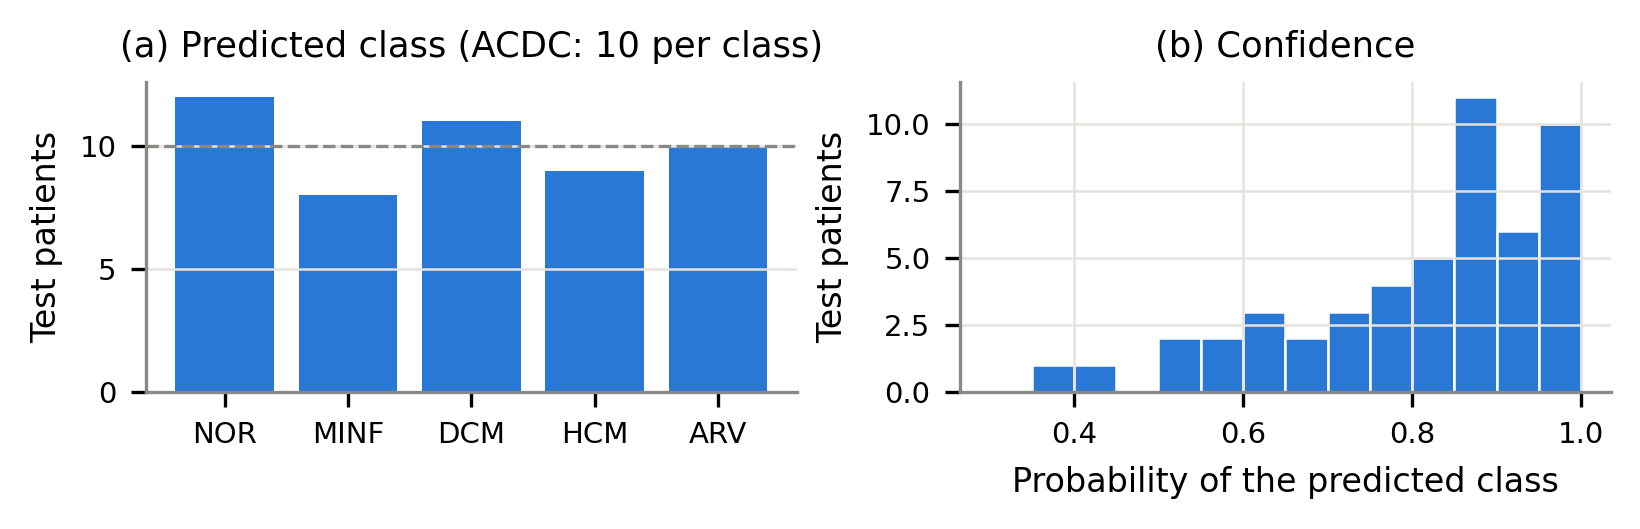
\includegraphics[width=\linewidth]{figs/supp/test_predictions.png}
  \caption{(a) Number of test patients predicted in each group by the final model; the dashed line marks the 10 patients per group of the ACDC test set. (b) Distribution of the probability of the predicted group.}
  \label{fig:supp-test}
\end{figure}

\clearpage
% ==========================================================================================
\section{Reproducibility}
\label{app:runs}

\subsection{Code organization}
The code is a Python package (data access, LV reconstruction, features, models, nested cross-validation, experiment tracking, figures) and six scripts run in order. Every run creates a timestamped folder with the configuration, library versions, log, metrics, tables (CSV and \LaTeX), figures and out-of-fold predictions; the latest successful run of each experiment is kept for the report. The data folders are only read.

\subsection{Experiments and running times}
% Generated by regenerate_supplementary.py from results/runs.csv
\begin{table}[H]
\centering
\small
\setlength{\tabcolsep}{4pt}
\begin{adjustbox}{max width=\linewidth}
\begin{tabular}{lcr}
\toprule
Experiment & Script & Time (min) \\
\midrule
Patient index, file checks & 1 & 0.1 \\
LV reconstruction on the training set & 2 & 0.3 \\
Features for every LV source & 3 & 0.7 \\
Protocol study (single split vs nested CV) & 4 & 14.3 \\
Benchmark (30 configurations, nested CV) & 5 & 48.8 \\
LV protocols (32 configurations) & 5 & 17.6 \\
Final model and test predictions & 6 & 6.9 \\
\bottomrule
\end{tabular}
\end{adjustbox}
\caption{Runs that produced the results of this report (Apple M3, 16 GB, 8 CPU cores; no GPU). Most of the time is spent training MLP ensembles inside the nested cross-validation.}
\label{tab:supp-runs}
\end{table}


\subsection{Software and parameters}
Python 3.12.6, NumPy 2.2.6, pandas 2.2.3, SciPy 1.14.1, scikit-learn 1.5.2, scikit-image 0.24.0, nibabel 5.3.2, PyTorch 2.6.0, XGBoost 3.0.0. Outer cross-validation: stratified 5-fold, 10 repeats (5 for the protocol study), seeds 0 to 9 (42 to 46 for the protocol study). Inner cross-validation: stratified 5-fold, accuracy as selection criterion, first configuration kept in case of ties (closest to 0.5 for $\alpha$). Logistic regression: multinomial, L2 penalty. SVMs: probabilities by Platt scaling with an internal 5-fold cross-validation. Random forests and extra trees: 300 trees. MLP ensemble: 50 networks, layer widths $d \to 32 \to 32 \to 32 \to 32 \to 5$, batch normalization (momentum 0.1), leaky ReLU (slope 0.01), cross-entropy, Adam with learning rate $10^{-3}$, 200 epochs, batches of 30, 75\% of the patients and $\lfloor 2d/3\rfloor$ features per network.

\stopcontents[appendix]
